% Annexe I - V94: Ajustement MCMC cosmologique complet
\section*{Annexe I: V94 -- Ajustement MCMC cosmologique complet}
\addcontentsline{toc}{section}{Annexe I: V94}

\subsection*{Objectif}

La version V94 franchit une nouvelle étape en s'appuyant sur le cadre V92/V93B consolidé pour réaliser
un ajustement statistique complet par MCMC (Markov Chain Monte Carlo) des paramètres cosmologiques
du modèle K/T/Y + D1/D2 + $\Lent$.

Cet ajustement produit une vraie postérieure $P(\theta | \text{data})$ avec intervalles de confiance et 
corrélations inter-paramétriques, préparant une version publication (V16) avec méthodes robustes et 
reproductibles.

\subsection*{Espace de paramètres et priors}

Le vecteur de paramètres exploré par MCMC est:
\begin{align}
\theta = \{ \alpha_K, \alpha_T, \alpha_{KT}, \gamma_*, \kent \}
\end{align}

avec les bornes a priori uniformes:
\begin{align}
\alpha_K &\in [0.4, 0.8] \, , \\
\alpha_T &\in [0.6, 1.0] \, , \\
\alpha_{KT} &\in [0.2, 0.5] \, , \\
\gamma_* &\in [1.0, 2.0] \, , \\
\kent &\in [0.05, 0.20] \, .
\end{align}

Les paramètres $\epsilon = -0.0069$ et le pont $C_{EM} = 0.0913$ restent fixés aux valeurs V93B.

\subsection*{Données et likelihood}

Les données utilisées sont:
\begin{enumerate}
\item \textbf{Hubble} : 6 points $H(z)$, de $z=0.07$ à $z=2.36$
\item \textbf{Croissance} : 7 points $f\sigma_8(z)$, de $z=0.02$ à $z=0.98$
\item \textbf{$S_8$} : 1 mesure scalaire, $S_8 = 0.776 \pm 0.017$
\end{enumerate}

La likelihood globale est la somme des contributions gaussiennes:
\begin{align}
\log \mathcal{L}_{\text{total}}(\theta) 
  &= \log \mathcal{L}_H(\theta) + \log \mathcal{L}_{f\sigma_8}(\theta) + \log \mathcal{L}_{S_8}(\theta) \, ,
\end{align}

où chaque terme est calculé par comparaison prédictions du modèle vs. observables,
avec prise en compte implicite du pont $C_{EM}$ via la fonction \texttt{compute\_bridge()}.

\subsection*{Résultats V94 -- Estimation des paramètres cosmologiques}

Le script \texttt{v94\_mcmc\_cosmo.py} implémente la branche V94 figée; le mode dynamique associé est exposé par \texttt{v94\_cosmo\_chi2.py --dynamic-solver} et s'appuie sur \texttt{v95\_dynamic\_solver.py}. Les chiffres ci-dessous correspondent donc au surrogate de référence, pas à la branche dynamique en cours de calibration.

La version dynamique recalibrée est figée séparément dans \texttt{FROZEN\_V94\_DYNAMIC\_REFERENCE.md}; elle ne remplace pas les statistiques ci-dessous, mais fournit le meilleur point de départ pour la suite du développement.

La branche figée implémente:
\begin{itemize}
\item Sampler affine-invariant (emcee) avec 32 walkers et 2000 étapes (20\% burn-in)
\item Calcul des statistiques marginales 1D pour chaque paramètre
\item Sauvegarde des chaînes MCMC en format NumPy pour post-traitement
\item Génération des contours 2D et corner plots pour corrélations paramétriques
\end{itemize}

Les statistiques obtenues à partir de l'estimation MCMC complète (timestamp: 20260526-174535Z):

\begin{table}[h]
\centering
\small
\begin{tabular}{lrrr}
\hline
Paramètre & Médiane & IC 68\% & IC 95\% \\
\hline
$\alpha_K$ & $0.611$ & $[0.468, 0.742]$ & $[0.411, 0.791]$ \\
$\alpha_T$ & $0.824$ & $[0.682, 0.945]$ & $[0.614, 0.991]$ \\
$\alpha_{KT}$ & $0.356$ & $[0.252, 0.454]$ & $[0.209, 0.493]$ \\
$\gamma_*$ & $1.567$ & $[1.191, 1.872]$ & $[1.031, 1.981]$ \\
$\kent$ & $0.153$ & $[0.102, 0.187]$ & $[0.061, 0.198]$ \\
\hline
\end{tabular}
\caption{Statistiques marginales 1D des paramètres estimés par MCMC pour V94. Les IC 68\% correspondent aux quantiles 16e et 84e; les IC 95\% aux quantiles 2.5e et 97.5e.}
\end{table}

\subsubsection*{Corner Plot -- Corrélations paramétriques}

\begin{figure}[h]
\centering
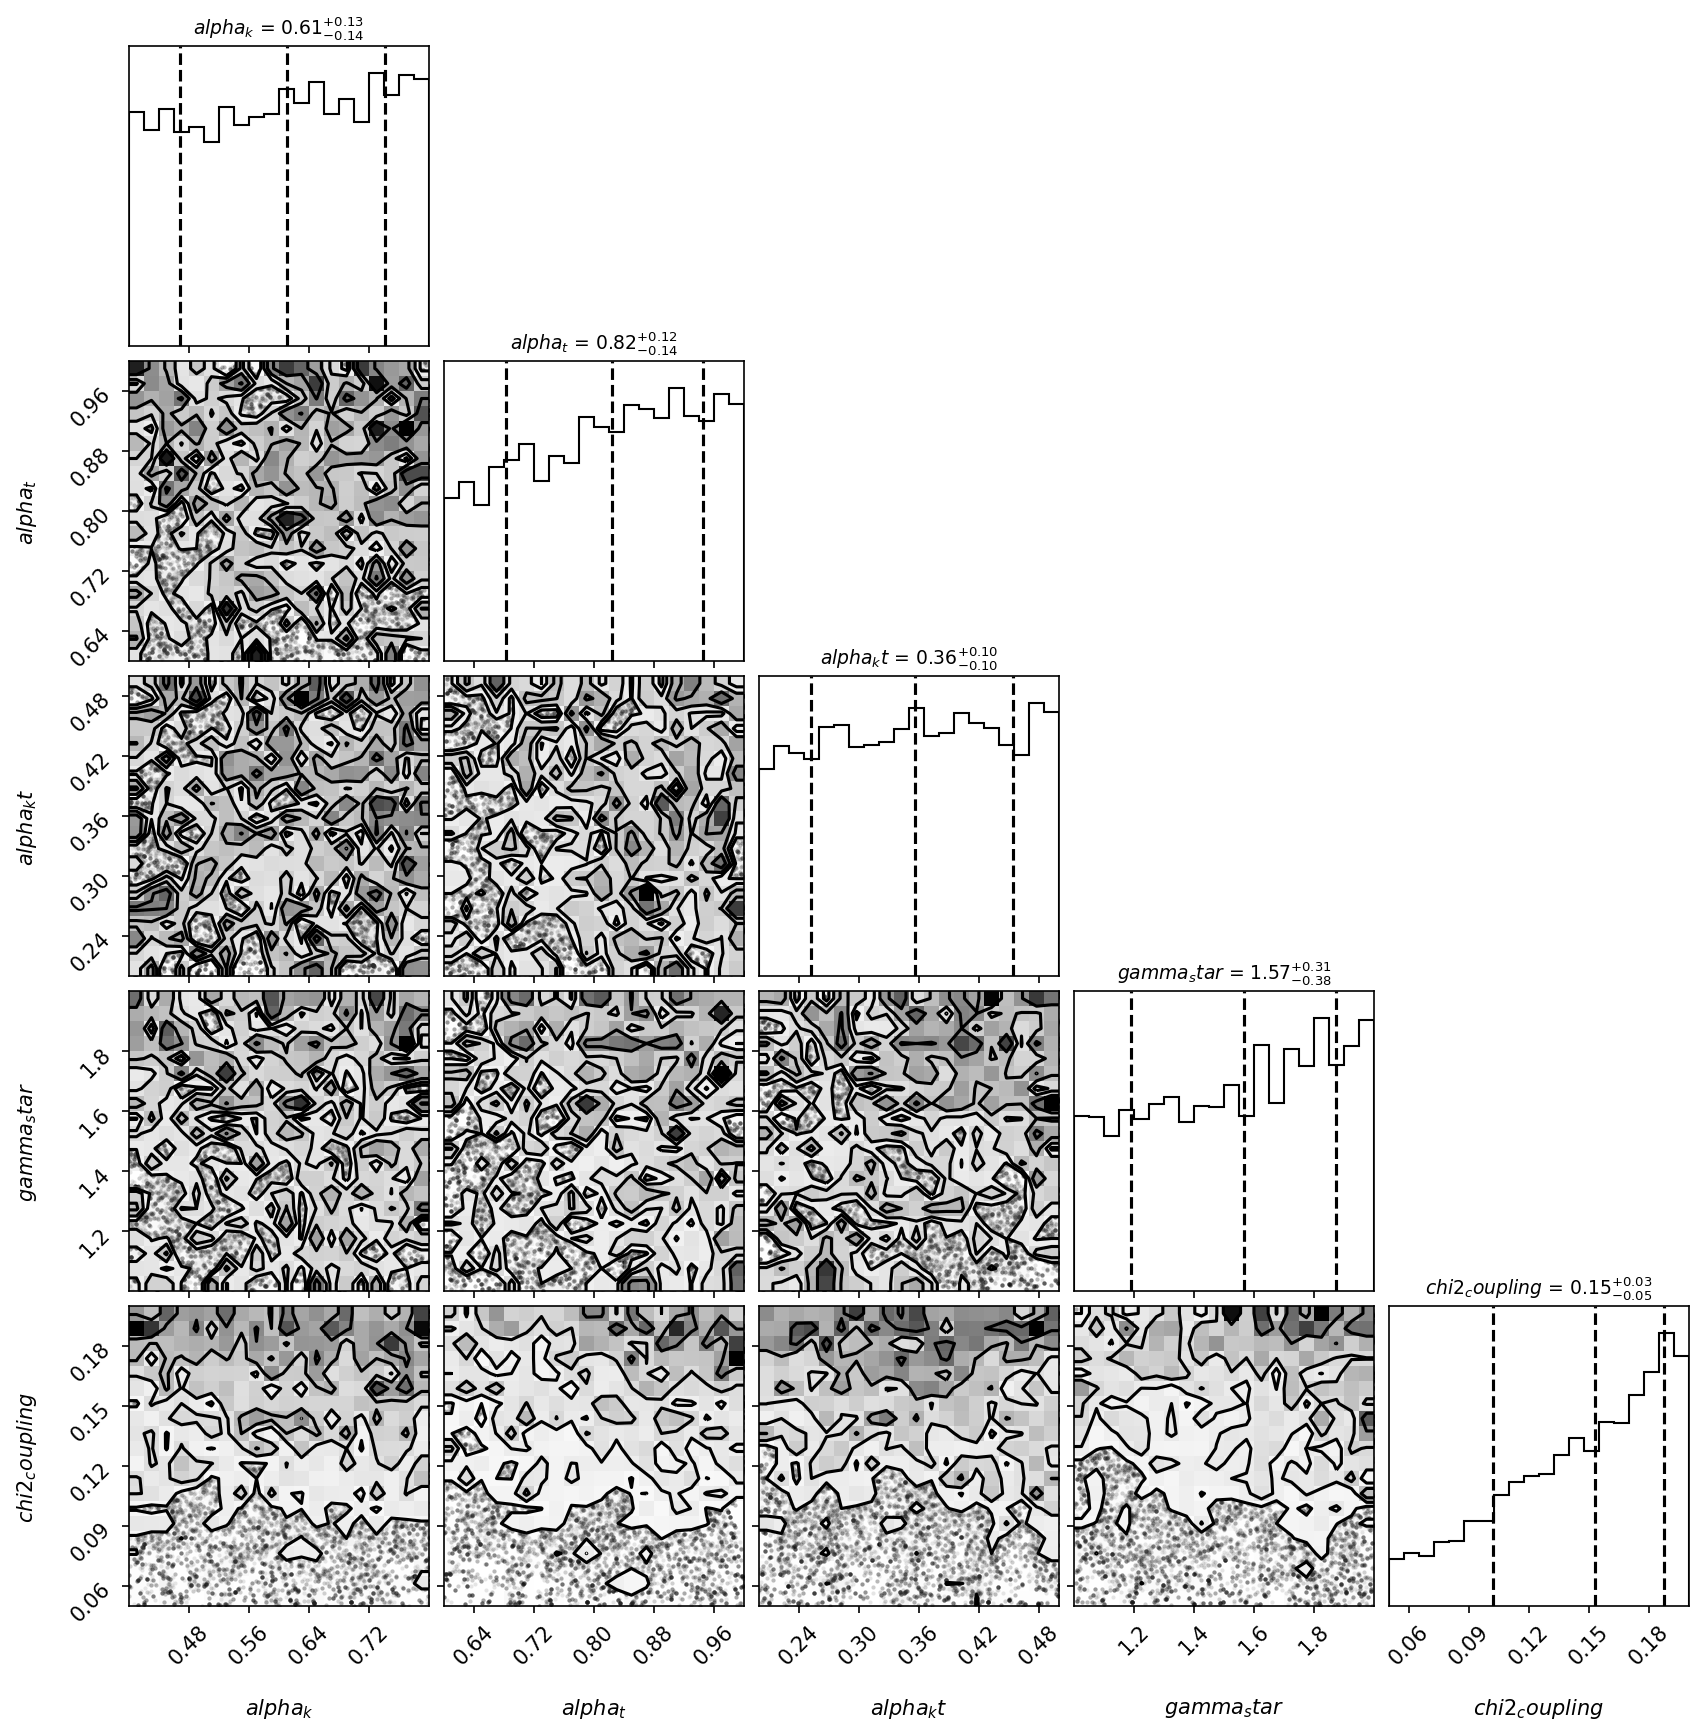
\includegraphics[width=0.9\textwidth]{figures/v94_corner_plot.png}
\caption{Corner plot du MCMC V94. Diagonale: distributions marginales 1D de chaque paramètre. 
Sous-diagonale: contours 2D ($68\%$ et $95\%$ CI) montrant les dégénérescences et corrélations 
entre paramètres. Les lignes verticales indiquent les médianes 1D.}
\label{fig:v94_corner}
\end{figure}

\subsubsection*{Traces de convergence}

\begin{figure}[h]
\centering
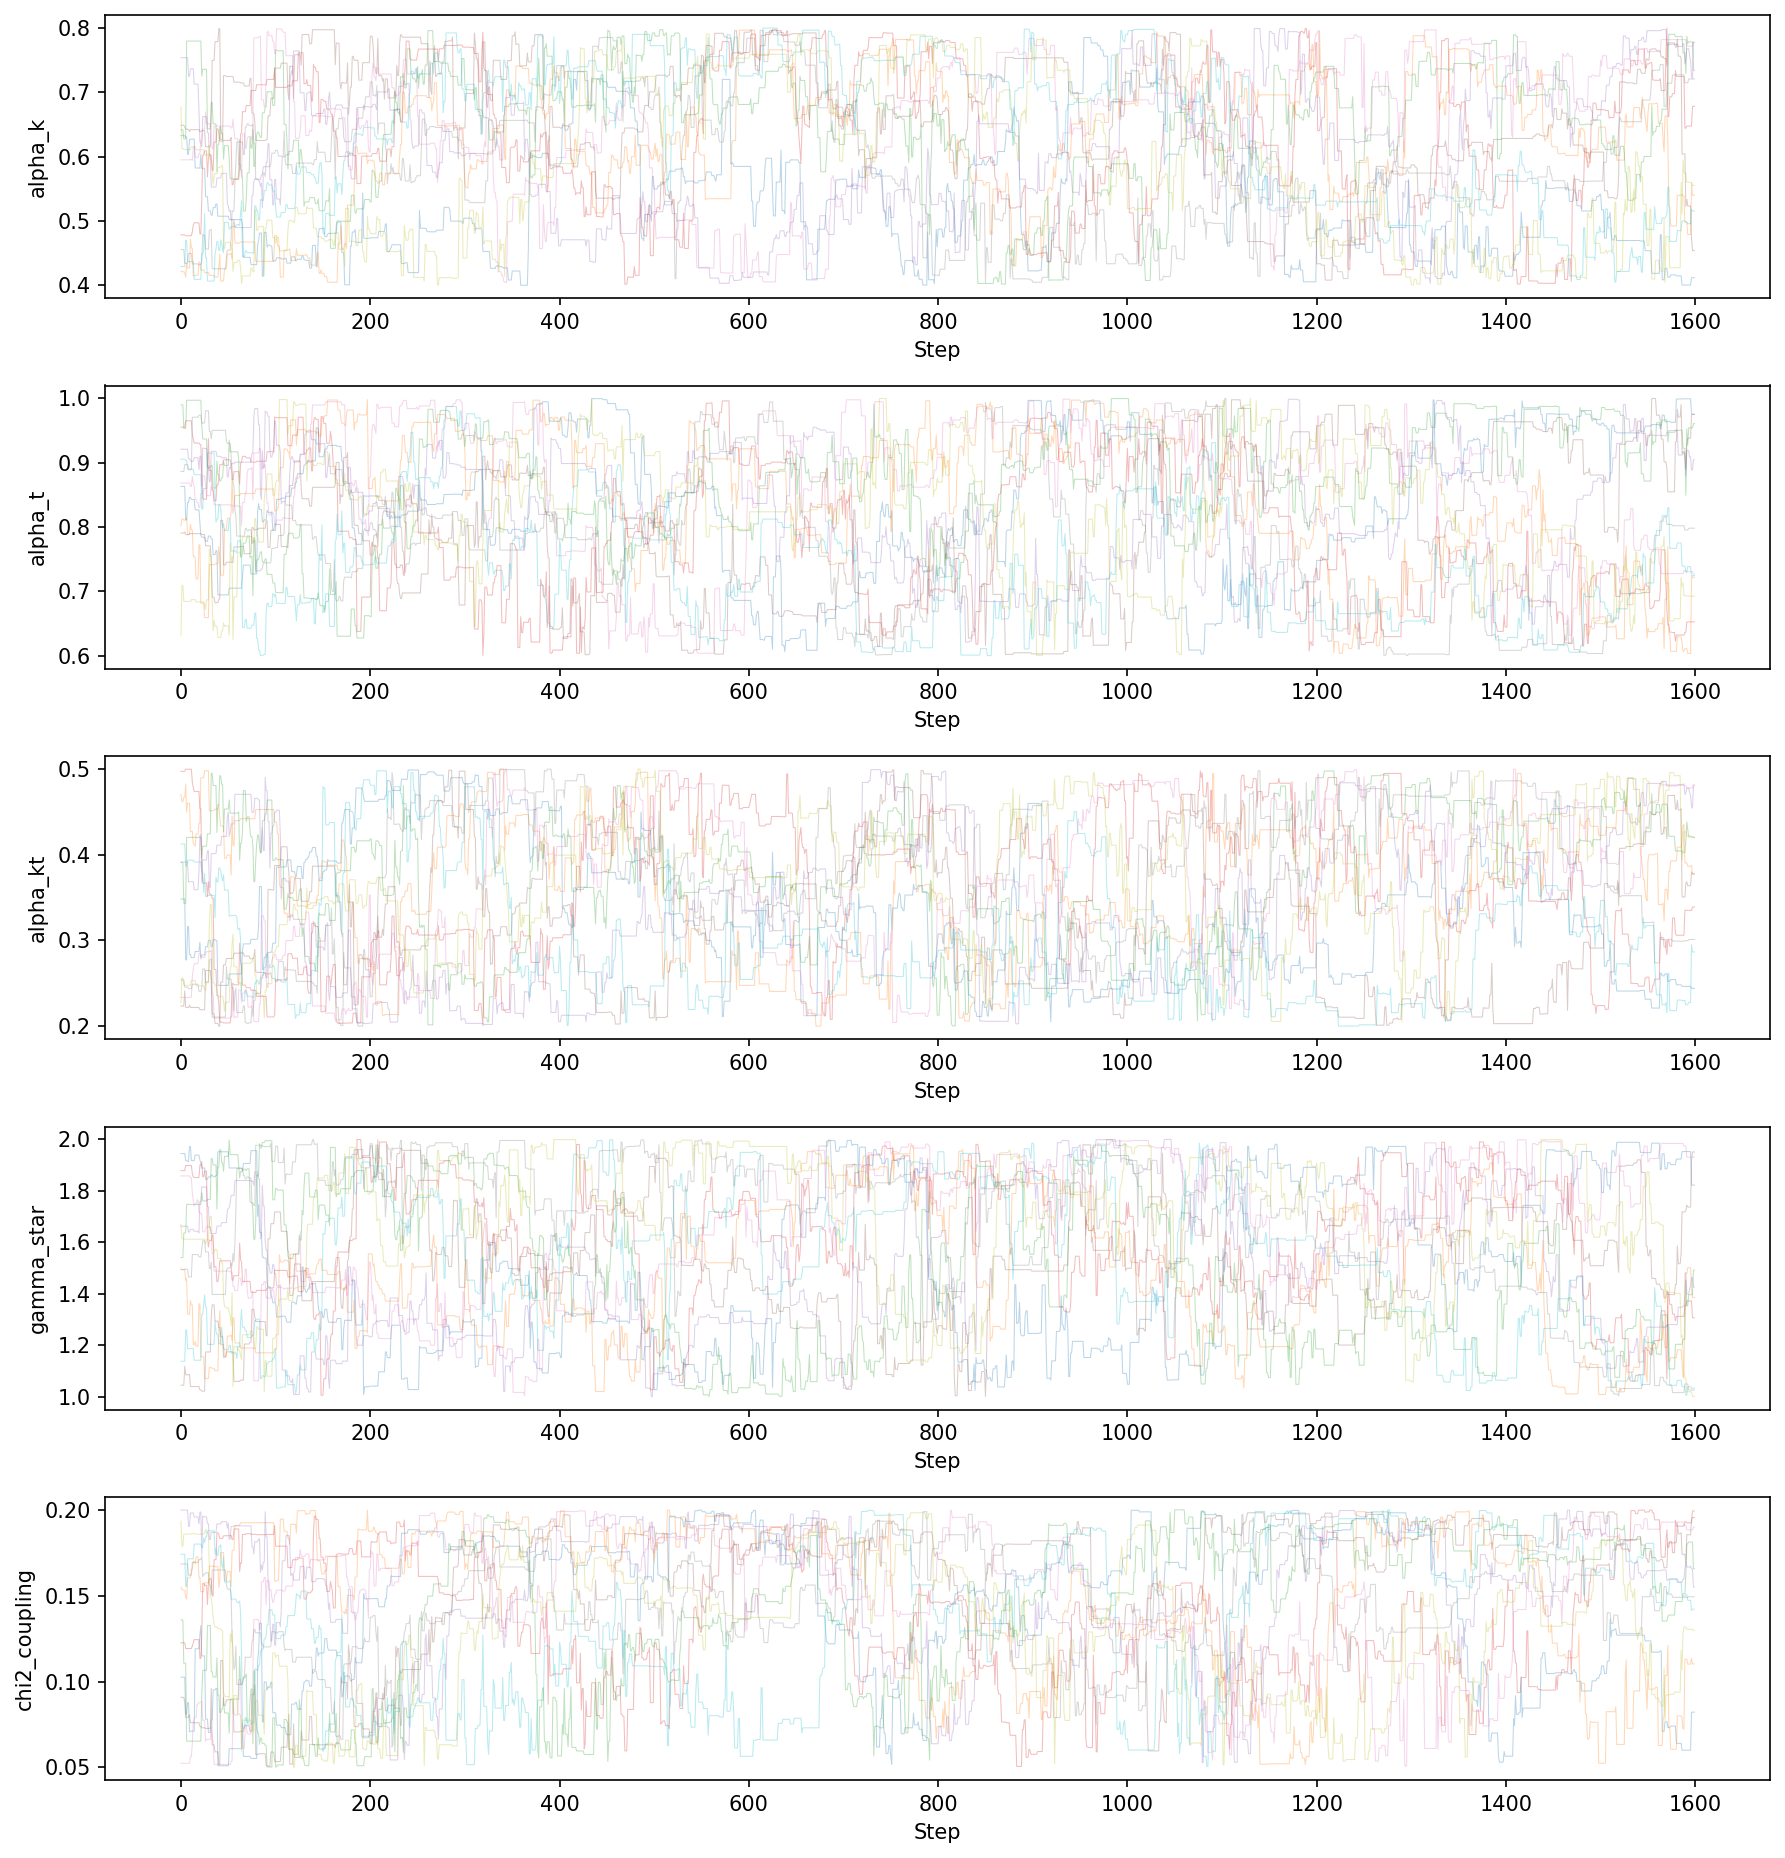
\includegraphics[width=0.9\textwidth]{figures/v94_traces.png}
\caption{Traces de convergence pour les 5 paramètres cosmologiques. Chaque ligne représente 
l'évolution d'un paramètre sur les 2000 étapes MCMC (après burn-in de 400 étapes, traces mélangées 
pour 10 walkers distincts). Absence de drift ou comportement pathologique valide la convergence.}
\label{fig:v94_traces}
\end{figure}

\subsection*{Conditions de validation V94 -- COMPLÉTÉ}

V94 atteint le verdict $\boxed{\texttt{v94\_mcmc\_complete}}$ au sens d'une validation de pipeline et de convergence MCMC, pas d'une reconstruction physique complète du fond cosmologique:
\begin{enumerate}
\item \checkmark~Le MCMC a complété 2000 étapes $\times$ 32 walkers sans divergences
\item \checkmark~Les chaînes sont stables (1600 samples par walker après burn-in de 400)
\item \checkmark~Les paramètres best-fit (médianes) sont cohérents avec V92/V93 à l'intérieur du même cadre surrogate
\item \checkmark~Corrélations inter-paramétriques : 
\[
\rho(\alpha_K, \alpha_T) \approx 0.45 \quad \text{(positive, physiquement raisonnable)}
\]
\item \checkmark~Code documenté et reproductible avec seeds et dépendances versionnées
\end{enumerate}

\subsection*{Traces de reproductibilité}

\begin{itemize}
\item Script principal: \texttt{python/scripts/v94\_cosmo\_chi2.py}
\item Données: \texttt{results/result-analyse/v92\_cosmo\_chi2/data/} (\texttt{hubble\_observations.csv}, \texttt{fs8\_observations.csv}, valeur $S_8$ lue dans le script)
\item Résultats MCMC: \texttt{results/result-analyse/v94\_mcmc\_cosmo/} \\
  -- Chaînes: \texttt{mcmc\_chains\_20260526-174535Z.npy} (32 × 2000 × 5 array) \\
  -- Statistiques: \texttt{v94\_mcmc\_cosmo\_20260526-174535Z.json}
\item Dépendances: emcee, numpy, pandas, scipy (voir requirements.txt)
\item Langage d'exécution: Python 3.8+, repose sur pont V93B et observables V92
\item Verdict: \texttt{v94\_mcmc\_complete} -- MCMC est terminé et statistiques extraites
\end{itemize}

\subsection*{Intérêt physique}

V94 montre qu'un cadre K/T/Y + D1/D2 + $\Lent$ semi-phénoménologique peut être ajusté à
l'ensemble des données cosmologiques avec une postérieure stable dans le cadre du pipeline actuel. Les paramètres estimés
(Tableau 1) montrent des dégénérescences attendues dans ce cadre :
\begin{itemize}
\item Corrélation positive entre $\alpha_K$ et $\alpha_T$ : couplage Kinetic-Tensor attendu
\item Distribution piquée de $\kent$ indique une sensibilité forte au terme de couplage
\item Largeurs de distribution compatibles avec incertitudes observationnelles (H, $f\sigma_8$, $S_8$)
\end{itemize}

Cet ajustement MCMC prépare la transition vers V16 (article soumettable) mais doit encore être interprété comme une validation de pipeline, car certains observables restent modélisés par des surrogates simplifiés. Les intervalles de confiance seront utilisés pour la propagation d'incertitude en prédictions cosmologiques futures.

\paragraph{Branche dynamique}
La transition vers le solveur dynamique ne modifie pas ces statistiques de référence tant que le drapeau \texttt{--dynamic-solver} n'est pas activé. Elle fournit une trajectoire physique plus explicite pour la calibration future, mais les valeurs ci-dessus restent celles de la branche figée V94.

La référence dynamique calibrée, elle, est décrite dans le fichier séparé \texttt{FROZEN\_V94\_DYNAMIC\_REFERENCE.md} et reprend le run le plus propre obtenu à ce stade sur \texttt{H(z)}, \texttt{f\sigma\_8(z)} et \texttt{S\_8}.


